\documentclass[a4paper,10pt,smallheadings,twocolumn]{scrartcl}

\usepackage{times}
\usepackage[T1]{fontenc}
\usepackage[utf8]{inputenc}
\usepackage{verbatimbox}
\usepackage[autostyle=true,german=quotes]{csquotes}
\usepackage{amsmath}
\usepackage{amsfonts}
\usepackage[top=2cm,right=2cm,bottom=3cm,left=2cm]{geometry}
\usepackage{fancyhdr}
\usepackage[lastpage,user]{zref}
\usepackage{multirow}
\usepackage{mathrsfs}
\usepackage{graphicx}
\usepackage{listings}
\usepackage{array}
\usepackage{multirow}
\usepackage{xcolor}
\usepackage{wrapfig}

\definecolor{mygreen}{rgb}{0,0.6,0}
\definecolor{mygray}{rgb}{0.5,0.5,0.5}
\definecolor{mymauve}{rgb}{0.58,0,0.82}

\newcommand{\Title}{Micro Controllers Summary}
\newcommand{\Author}{Lucien Zürcher}
\newcommand{\Date}{\today}

\newcommand{\norm}[1]{\lvert\lvert #1 \rvert\rvert}

\title{\vspace{-1cm}\Title\vspace{0cm}}
\date{\Date}
\author{Lucien Zürcher}

\graphicspath{ {./assets/} }

\pagestyle{fancy}
\fancyhf{}
\fancyhead[L]{\Title}
\fancyhead[R]{\Author}
\fancyfoot[L]{MC}
\fancyfoot[C]{\Date}
\fancyfoot[R]{Page \thepage\ of \zpageref{LastPage}}
\renewcommand{\headrulewidth}{0.4pt}
\renewcommand{\footrulewidth}{0.4pt}

\setlength{\columnsep}{1cm}
\setlength{\parindent}{0cm}
\setcounter{MaxMatrixCols}{20}

\makeatletter
\newenvironment{multicases}[1]
  {\let\@ifnextchar\new@ifnextchar
   \left\lbrace\def\arraystretch{1.2}%
   \array{@{}l*{#1}{@{\quad}l}@{}}}
  {\endarray\right.\kern-\nulldelimiterspace}
\makeatother

% minimize spacing of lists
\usepackage{enumitem}
\setitemize{noitemsep,topsep=0pt,parsep=0pt,partopsep=0pt}
\setenumerate{noitemsep,topsep=0pt,parsep=0pt,partopsep=0pt}

\newenvironment{tightenumerate}{
\begin{enumerate}
    \setlength{\itemsep}{0pt}
    \setlength{\parskip}{0pt}
}{\end{enumerate}}

\newenvironment{tighitemize}{
\begin{itemize}
    \setlength{\itemsep}{0pt}
    \setlength{\parskip}{0pt}
    \renewcommand\labelitemi{-}
}{\end{itemize}}

\lstdefinestyle{customc}{
  belowcaptionskip=1\baselineskip,
  breaklines=true,
  frame=L,
  xleftmargin=\parindent,
  language=C,
  showstringspaces=false,
  basicstyle=\footnotesize\ttfamily,
  keywordstyle=\bfseries\color{green!40!black},
  commentstyle=\itshape\color{purple!40!black},
  identifierstyle=\color{blue},
  stringstyle=\color{orange},
}

\lstdefinestyle{customasm}{
  belowcaptionskip=1\baselineskip,
  frame=L,
  xleftmargin=\parindent,
  language=[x86masm]Assembler,
  basicstyle=\footnotesize\ttfamily,
  commentstyle=\itshape\color{purple!40!black},
}

\lstset{escapechar=@,style=customc}

\begin{document}

\maketitle
\thispagestyle{fancy}
\tableofcontents
\clearpage

\section{System Components}

\subsection{Von Neumann Architecture}

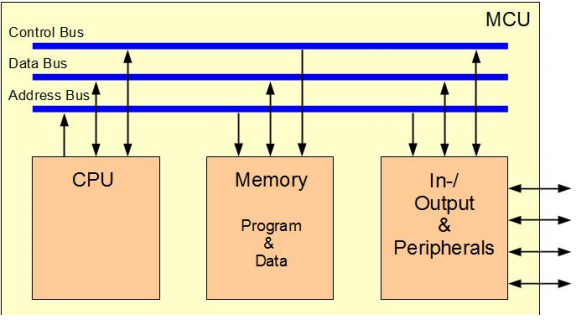
\includegraphics[width=0.5\textwidth]{von-neumann-architecture.png}

\textit{Components:}

\begin{itemize}
    \item{\textbf{CPU}, Central Processing Unit}
    \item{\textbf{Memory}, Program and Data}
    \item{\textbf{In-/Output}-Unit, Peripherals}
    \item{\textbf{Bus}-System: Communication}
\end{itemize}

\textit{One \textbf{shared bus and memory} for program and data.}

\subsection{Harvard-Architecture}

\textit{
    basically same as Von Neumann, with the difference, that
    there are \textbf{two separate bus systems} for program and data
}

\subsection{Numerical Systems}

\textit{
    Numerical value $Z_B$ of a n-digit, integer number with base $B$ ($B \geq 2$):
}

\begin{center}
    $Z_B = \sum^{n-1}_{i=0} x_i \cdot B^i$
\end{center}

\begin{tabular}{c|c|c}
    \hline
    \textbf{Decimal}  & \textbf{Dual / Binary}         & \textbf{Hexadecimal} \\
    197               & 0b1100'0101                    & 0xC5 \\
    $B=10$            & $B=2$                          & $B=16$ \\
    & & \\
    $=1 \cdot 10^2 +$ & $=1 \cdot 2^7 + 1 \cdot 2^6 +$ & $=C \cdot 16^1 + 5 \cdot 16^0$ \\
    $9 \cdot 10^1 +$  & $ 0 \cdot 2^5 + 0 \cdot 2^4 +$ & $=12 \cdot 16^1 + 5 \cdot 16^0$ \\
    $7 \cdot 10^0 $   & $ 0 \cdot 2^3 + 1 \cdot 2^2 +$ & \\
                      & $ 0 \cdot 2^1 + 1 \cdot 2^0 $  & \\
    \hline
\end{tabular}
\\
\textit{The amount of presentable numbers is $B^n$}
\textit{
    The highest presentable number is $B^n-1$.
    Calculated from $x_i = B - 1$ for $n-1 \geq i \geq 0$
}

\subsection{hex / binary}

\begin{tabular}{rrl|rll}
    H   & D   & B       &  Dec   & Bin \\
    \hline
    $0$ & $0$ & $0000$  & 16     & $2^5$    & (max 31)      \\
    $1$ & $1$ & $0001$  & 32     & $2^6$    & (max 63)      \\
    $2$ & $2$ & $0010$  & 64     & $2^7$    & (max 127)     \\
    $3$ & $3$ & $0100$  & 128    & $2^8$    & (max 255)     \\
    $4$ & $4$ & $0101$  & 256    & $2^9$    & (max 511)     \\
    $5$ & $5$ & $0110$  & 512    & $2^{10}$ & (max 1'023)   \\
    $6$ & $6$ & $0111$  & 1'024  & $2^{11}$ & (max 2'047)   \\
    $7$ & $7$ & $1000$  & 2'048  & $2^{12}$ & (max 4'095)   \\
    $9$ & $9$ & $1001$  & 4'096  & $2^{13}$ & (max 8'191)   \\
    $A$ & $10$ & $1010$ & 8'192  & $2^{14}$ & (max 16'383)  \\
    $B$ & $11$ & $1011$ & 16'384 & $2^{15}$ & (max 31'767)  \\
    $C$ & $12$ & $1110$ & 32'768 & $2^{16}$ & (max 65'535)  \\
    $D$ & $13$ & $1011$ & \\
    $E$ & $14$ & $1011$ & \\
    $F$ & $15$ & $1011$ & \\
\end{tabular}

\subsection{Signed numbers}

\textit{two's compliment is beeing used}

\begin{center}
$Z_{signed} = -x_{n-1} \cdot 2^{n-1} + \sum^{n-2}_{i=0} x_i \cdot 2^i$
\end{center}

\textit{most significant bit is negative}

\textit{Example: $-1$ as 16-bit Hex = $0xFFFF$}
\\
\textit{
    Conversion:
    \begin{enumerate}
        \item{Invert binary  : $-6 \rightarrow 0110 \rightarrow 1001$}
        \item{increment by 1 : $1001 + 0001 \rightarrow 1010$}
    \end{enumerate}
}

\begin{tabular}{rrl|rll}
\end{tabular}

\subsection{carry / overflow}

\begin{tabular}{p{0.2\textwidth}p{0.2\textwidth}}
    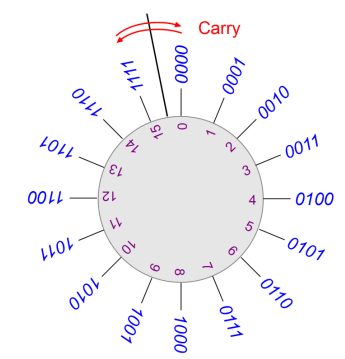
\includegraphics[width=0.2\textwidth]{carry-circle.png} &
    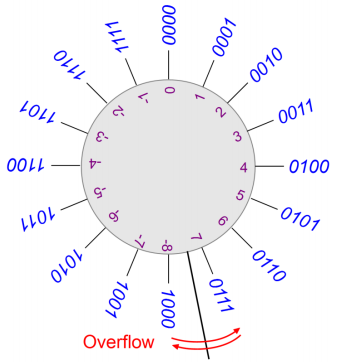
\includegraphics[width=0.2\textwidth]{overflow-circle.png} \\
    \textit{
        \textbf{Carry} is set on crossover between lowest
        and highest number
    } &
    \textit{
        \textbf{Overflow} happens on crossover between
        highest absolut values
    } \\
\end{tabular}

\subsection{Bit groups}

\textit{
    \textbf{Nibble/Tetrade} has the size of 4 bits
}

\textit{
    \textbf{Byte} has the size of 8 bits
}

\textit{
    \textbf{Word} is MC9S08JM60 specific, it has 16 bits
}

\pagebreak
\subsection{Quantity of address lines}
\begin{wrapfigure}{l}{0.2\textwidth}
    \centering
    \hspace{-20pt}
    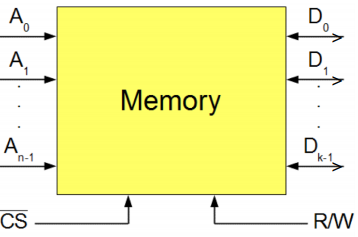
\includegraphics[width=0.2\textwidth]{memory.png}
    \hspace{-50pt}
\end{wrapfigure}

\textit{$\mathbf{n}$ Quantity of address lines} \\
\textit{$\mathbf{2^n}$ Quant. of storage locations} \\
\textit{$\mathbf{2^n \cdot k}$ Quant. of bits in memory}
\\
\\
\begin{tabular}{rcrcrcr}
    1 K  & = & $2^{10}$ & = &  1024 Bit & \^= & 10 Adresslines \\
    64 K & = & $2^{16}$ & = & 65536 Bit & \^= & 16 Adresslines \\
\end{tabular}
\\ \\
\textit{example, $32K \times 8$ memory storage space:}
\\ \\
\textit{
    \textbf{bits storage}: $32 \cdot 2^10 \cdot 8 = 2^5 \cdot 2^10 \cdot 2^3 = 2^18 \rightarrow 18$ Bits \\
    \textbf{number address lines}: $32 \cdot 2^10 = 2^15 = 32 768$ \\
    \textbf{highest address}: $2^{18}-1 = 0x7FFFF = 262'143$
}

\subsection{Microprocessor vs Mircocontroller}

\textit{
    \textbf{Mircocontroller} contains CPU (Processor), Peripherals (I/O)
    and Memory (RAM / ROM). Basically a small computer.
}
\\
\textit{
    \textbf{Mircoprocessor} has only CPU and som integrated Circuits.
}

\subsection{CPU components}

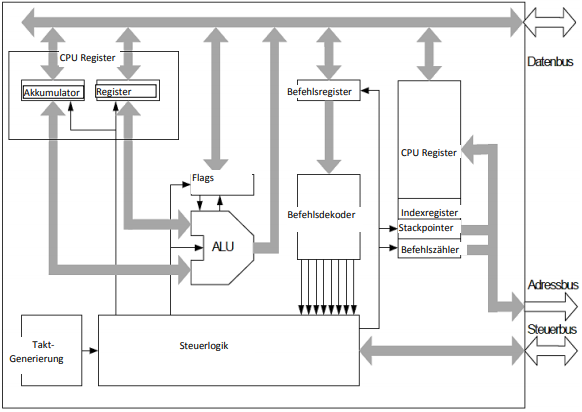
\includegraphics[width=0.5\textwidth]{cpu-overview.png}

\textit{
    ALU (Aritmetic Unit), AKKU (Accumulator), PC (Programming Counter),
    Busses, Instruction-Register, Address-Register,
    Operand-Register, Control Unit, ..
}

\subsection{Instruction Cycle Steps}

\begin{enumerate}
    \item{instruction fetch}
    \item{instruction decode}
    \item{(operand fetch)}
    \item{instruction execute}
    \item{next address and inc PC}
\end{enumerate}

\subsection{Types of MCU Registers}

\textit{
    AKKU, PC, Instruction-Register (decoder), Operand-Register
}

\section{Compiling}

\subsection{Codewarrior Designflow}

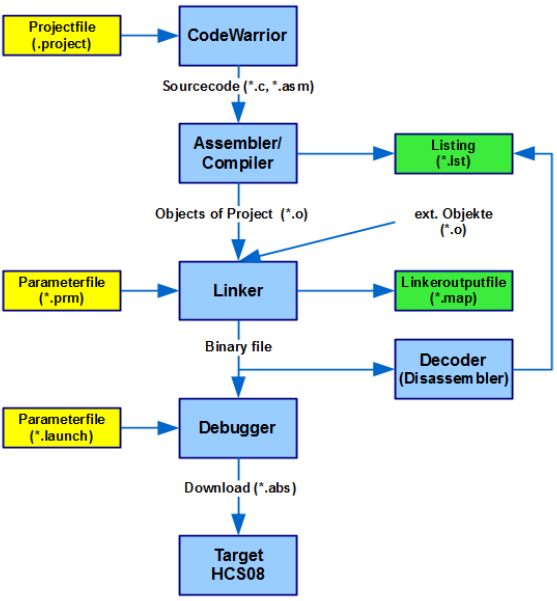
\includegraphics[width=0.5\textwidth]{codewarrior-designflow.png}

\subsection{Programming Language}

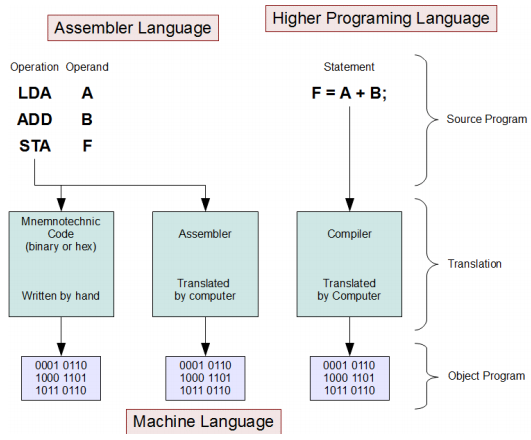
\includegraphics[width=0.5\textwidth]{programming-languages.png}

\textit{High level programming languages are:}

\begin{itemize}
    \item{portable}
    \item{efficient (normaly)}
    \item{Better readable}
    \item{easier to maintain}
\end{itemize}

\textit{
    High level programming languages are usually prefered,
    if enough computational power and memory is available.
}
\\
\textit{
    Assembler is often used, if the application:
}
\begin{itemize}
    \item{is time critical and needs exact timing}
    \item{timing of the high level programming language to unpredictible is}
\end{itemize}

\subsection{Assembler Code-Format}

\begin{tabular}{rllll}
        & \textbf{Label}  & \textbf{Instruction}  & \textbf{Operands} & \textbf{comment} \\
    Ex1 & Limit: & EQU          & \$CD       & ; define limit \\
    Ex2 & Start: & LDA          & \#Limit     & ; load limit \\
\end{tabular}

\textit{
    \textbf{Instruction}: is a command for the processor
} \\
\textit{
    \textbf{Directive}: are instructions that direct the assembler /
    compiler to do something
}

\begin{tabular}{rlll}
        & \textbf{Type} & \textbf{Directed to}  & \textbf{Results in program code} \\
    \hline
    Ex1 & \textbf{Instruction} & Target CPU     & Yes \\
    Ex2 & \textbf{Directive}   & Assembler      & Only indirect \\
        & \textbf{Comment}     & Programmer     & No \\
\end{tabular}

\subsection{Parameter file}

\textit{
    The Parameter file (*.prm) is used for by the Linker. It takes the machine
    code and defines the location on the controller. It is important,
    so that jumps work correctly.
    It contains:
}

\begin{itemize}
    \item{Memory-Map of the Prozessor (Location and size of Flash, RAM, ..)}
    \item{Extra definitions, where which parts of the code on the Controller should be located}
\end{itemize}

\section{Assembler \& HCS08}

\subsection{HCS08 CPU Registers}

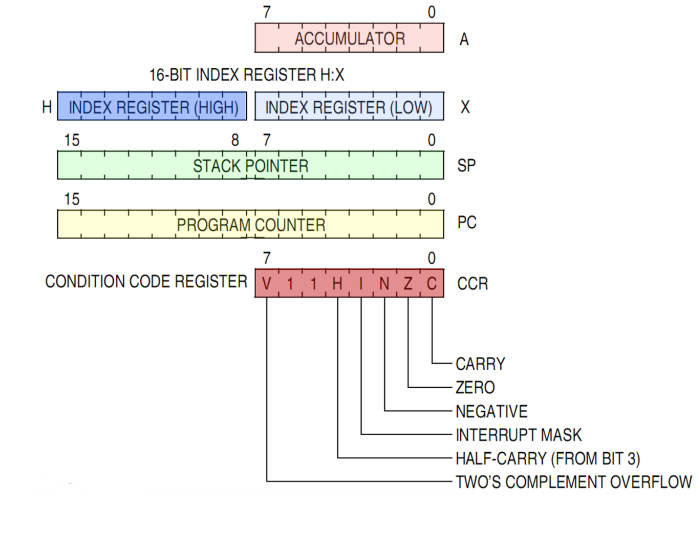
\includegraphics[width=0.5\textwidth]{hcs08-cpu-registers.png}

\textit{
    Registers the HCS08 contains:
}

\begin{itemize}
    \item{HX Register}
    \item{PC}
    \item{Akku}
    \item{Stack Pointer}
    \item{CCR}
\end{itemize}

\subsection{HCS08 Processor}

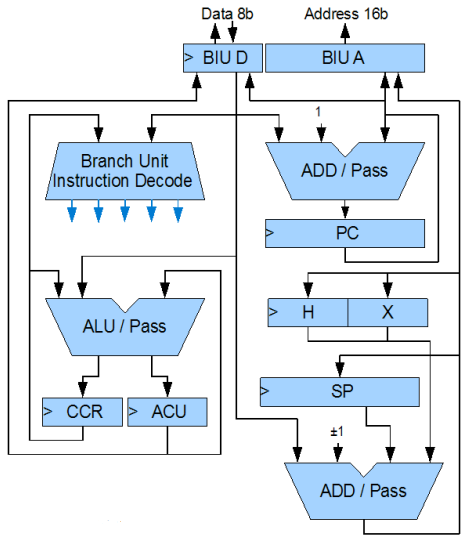
\includegraphics[width=0.5\textwidth]{hcs08-overview.png}

\begin{itemize}
    \item{8 Bit, Von Neumann archidecture}
    \item{\textbf{BIU} Bus Interface Unit}
    \item{\textbf{PC} Program Counter}
    \item{\textbf{ACU} Accumulator}
    \item{\textbf{ALU} Arithmetic Logic Unit}
    \item{\textbf{CCR} Condition Code Register (Collection of status flags)}
    \item{\textbf{SP} Stack (LI-FO, Pointer for Context and Parameter)}
    \item{\textbf{H:X} Index Register}
\end{itemize}

\subsection{Memory Mapping}

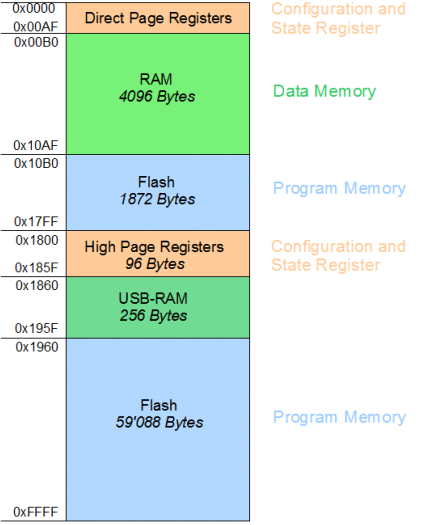
\includegraphics[width=0.5\textwidth]{hcs08-memory-mapping.png}

\textit{
    Access to the directpage (0x0000 - 0x0AF) needs less cycles,
    since the address is only 1 Bytes long.
}

\subsection{Register configuration HCS08}

\begin{lstlisting}
// define the dataflow direction input = 0 | output = 1
PTADD = 0x04;

// set output value
PTAD = 0x04;
// read value
uint_8 val = PTAD;

// set pullup enable port
PTADD = 0x00;
PTAPE = 0x04;
\end{lstlisting}

\begin{tabular}{rl}
    \textbf{Reg. Name} & \textbf{Description} \\
    PTxDD & \textit{Data Direction of Port x} \\
    PTxD  & \textit{Data value of Port x} \\
    PTxPE & \textit{Set Pullup Enable of Port x} \\
          & \textit{(PTxDD needs to be 0)} \\
\end{tabular}

\textit{
    \textbf{Pullup Enable} is used to pullup the value
    of the output to 1. This is usually used on a bus system
    to prevent a short circuit.
}

\subsection{Differences of Operations}

\textit{
    Comparing different operations, following should be taken
    in consideration:
}

\begin{itemize}
    \item{number of cycles}
    \item{memory usage, 8bit (directpage) / 16bit}
    \item{Set CCR bits / flags}
    \item{Used registers}
    \item{Address modes}
\end{itemize}

\section{Assembler Directives \& Addressing Modes}

\subsection{Directives}

\begin{tabular}{lp{0.3\textwidth}}
    \textbf{Directive} & \textbf{Description} \\
    $\mathbf{SECTION}$ & \textit{Defines the beginning of a relocatable section} \\
    $\mathbf{EQU}$     & \textit{Assigns an expression to a name. Not redefinable} \\
    $\mathbf{DC}$      & \textit{Defines one or more constants and their names. Will be stored at the set location} \\
    $\mathbf{DS}$      & \textit{Allocates memory(RAM) for variables} \\
\end{tabular}

\textit{
    The Assembler-Directive $\mathbf{SECTION}$ defines program- and
    data section. Those section can be moved freely within the memory (relocative
    assembling), \textbf{after} the \textbf{assembly} process is finished. \\
    The final memory area location happens after the linking process. The locations
    of those sections can therefor be defined in the \textbf{Linker-Parameterfile}.
}

\subsection{Basic Assembler Program}

\begin{lstlisting}
; include definitions
include 'MC9S08JM60.inc'

; -- globals
GLOBAL _Startup ; define start of programm
GLOBAL main
GLOBAL dummy    ; Dummy Interrupt Service Routine

; -- equations
StackSize: EQU   $60   ; stack size
pi:        EQU   31416 ; example of random equ

; -- stack
DATA_STACK: SECTION
TofStack:  DS    StackSize-1 ; definiton of "Top of Stack"
BofStack:  DS    1           ; definition of "Bottom of Stack"

; -- create space for data
DATA:   SECTION
var1:   DS    1   ; Example of a 1 Byte Variable
Array1: DS    $20 ; Example of an Array of $20 Bytes

; -- setup constants
CONST:     SECTION
Maske1:      DC.B    %00000001
Parameter1:  DC.B    $3A    ; DC with a point
Parameter2:  DC.W    57100  ; word with int value
Reserve_Par: DS      16     ; reserve empty 16 Bytes
VarArray:    DS.W    3      ; reserve 3 Words
STRING1:     DC.B    10,"Hello",$0D

; -- program start (initialisation)
PROGRAMM:   SECTION ; Code Segment
_Startup:           ; Resetvektor points to this
Stackinit:  LDHX  #(BofStack+1)
            TXS          ; decrement TXS, thats why +1 BofStack
            LDA   #$00
            STA   SOPT1  ; Disable Watchdog

; -- actual program
main:
    ; turn on backligths of the car
    BSET    PTDD_PTDD2, PTDD
    BSET    PTDDD_PTDDD2, PTDDD

    CLR     RamLoc

    BCLR    PTGDD_PTGDD0, PTGDD
    BCLR    PTGDD_PTGDD1, PTGDD
    BCLR    PTGDD_PTGDD2, PTGDD
EndlessLoop:
    ; load joystick values
    MOV     RamLoc, PTGD
    JMP     EndlessLoop

; (=ensure program end if endlessloop is missing)
EndLoop:    BRA     *

; catch any unexpected interrupts
dummy:          BGND
                BRA     dummy

\end{lstlisting}

\subsection{Addressing Modes}

\begin{itemize}
    \item{\textit{\textbf{Immediate}: 1 Byte operand in instruction (LDA \#\$01)}}
    \item{\textit{\textbf{Inherent}: no operand required (e.g. NOP, INCA..)}}
    \item{\textit{\textbf{Direct}: onlu direct page, 1 address Byte}}
    \item{\textit{\textbf{Extended}: whole 64k area, 2 address Bytes}}
    \item{\textit{\textbf{Indexed}: with SP (Stack pointer) or HX (7 sub modes)}}
    \item{\textit{\textbf{Relative}: for branches, PC=PC+2+two's compl.}}
\end{itemize}

\textit{
    Different addressing modes of the same instruction type use differnet
    operation codes (e.g. LDA-MM: A6; LDA-DIR: B6). \\
}

\subsubsection{Immediate (IMM)}

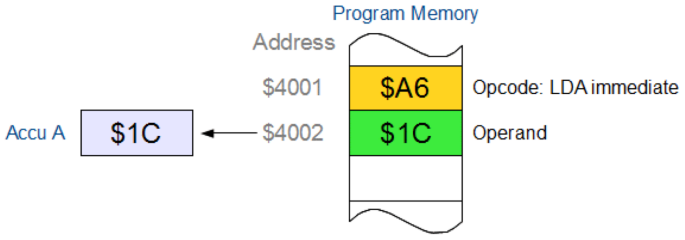
\includegraphics[width=0.5\textwidth]{addressmode-immediate.png}

\textit{
    \textbf{Immediat adressing} mode: the following Byte of the operation code
    is immediately used as the operand. \\
    Example: \textbf{LDA \#\$1C}
}

\subsubsection{Inherent (INH)}

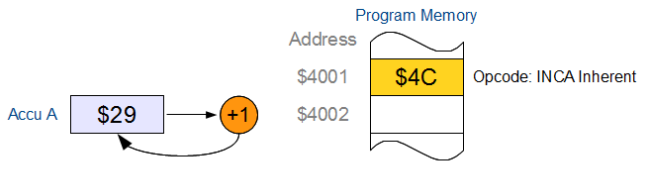
\includegraphics[width=0.5\textwidth]{addressmode-inherent.png}

\textit{
    \textbf{Inherent addressing} mode: no explicit operand address needed.
    All operands are in the CPU-registers \\
    Example: \textbf{INCA}
}

\subsubsection{Direct (DIR)}

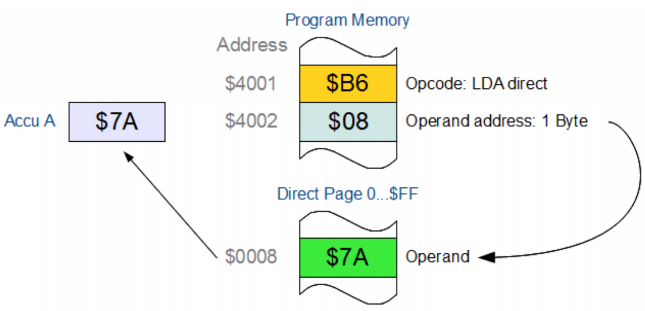
\includegraphics[width=0.5\textwidth]{addressmode-direct.png}

\textit{
    \textbf{Direct addressing} mode: After the operation code, the
    \textbf{1-Byte} operand address follows in the program memory. \\
    Only operands in the address section between \$00 and \$FF are
    supported. (The Direct Page Registers 0x00-0xAF, Direct Page RAM 0xB0-0xFF) \\
    Example: \textbf{LDA \$08}
}

\subsubsection{Extended (EXT)}

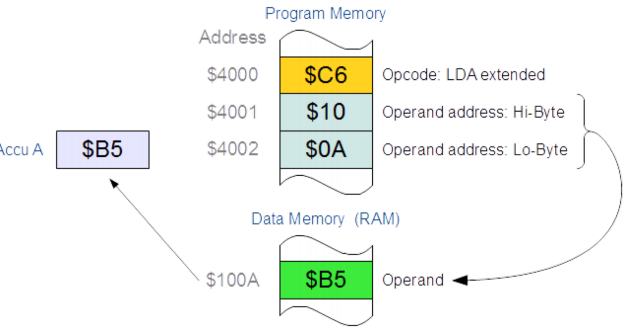
\includegraphics[width=0.5\textwidth]{addressmode-extended.png}

\textit{
    \textbf{Extended addressing} mode: After the operation code, the \textbf{2-Byte}
    operand address follows in the program memory. \\
    Supports the whole address section between 0x0000 - 0xFFFF. But is also slower. \\
    Example: \textbf{LDA \$34,X}
}

\subsubsection{Indexed (IX1)}

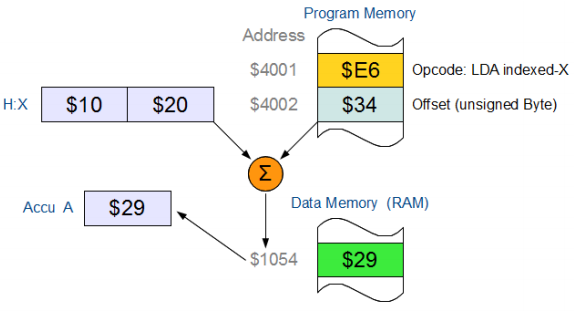
\includegraphics[width=0.5\textwidth]{addressmode-indexed.png}

\textit{
    \textbf{Indexed addressing} mode: uses the \textbf{HX} or \textbf{SP} register. \\
    Through indexed addressing the final assigned operand address is dependent from
    the program behaviour (address arithmetics).
}

\textit{Following are sub modes of the indexed addressing mode}

\begin{tabular}{lp{0.25\textwidth}l}
    $\mathbf{IX}$   & \textit{Indexed addressing with H:X, without offset}
                    & \scriptsize{\textbf{LDA  X}} \\
    $\mathbf{IX1}$  & \textit{Indexed addressing with H:X and \textbf{8-bit offset}}
                    & \scriptsize{\textbf{LDA  \$34, X}} \\
    $\mathbf{IX2}$  & \textit{Indexed addressing with H:X and \textbf{16-bit offset}}
                    & \scriptsize{\textbf{LDA  \$34A5, X}} \\
    $\mathbf{IX+}$  & \textit{
                            Indexed addressing with \textbf{H:X} and \textbf{H:X
                            Increment}. Only for MOV and CBEQ
                            (Compare Accu with value on the address that
                            is stored in the H:X register. If values are
                            equal, jump to Label and increment H:X)
                            instructions
                        }
                    & \scriptsize{\textbf{CBEQ  X+, Label}} \\
    $\mathbf{IX1+}$ & \textit{Same as IX+, with \textbf{Increment} and \textbf{8-bit offset} (Only available for instruction CBEQ)}
                    & \scriptsize{\textbf{CBEQ  \$34,X+, Label}} \\
    $\mathbf{SP1}$  & \textit{Same as IX1, but with Stackpointer SP instead of H:X.}
                    & \scriptsize{\textbf{LDA  \$34, SP}} \\
    $\mathbf{SP2}$  & \textit{Same as IX2, but with Stackpointer SP instead of H:X.}
                    & \scriptsize{\textbf{LDA  \$34A5, SP}} \\
\end{tabular}

\subsubsection{Relative (REL)}

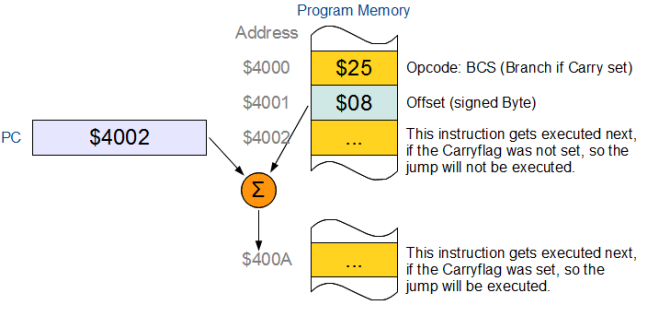
\includegraphics[width=0.5\textwidth]{addressmode-relative.png}

\textit{
    \textbf{PC relative addressing} mode: is only used with BRANCH-Instructions. \\
    The following Byte after the operand is a \textbf{two's complement} offset
    to the already increased program counter. \\
    The address range with relaive addressing is -126 to +129. 129, since
    the PC is incremented before and after the jump (+2).
}


\newpage

\end{document}
